\chapter{Ausblick}

\textbf{Diese Kapitel ist noch under Konstruktion ;)}

Nobelpreis in Chemie 2017, "Für die Entwicklung der Kryo-Elektronenmikroskopie, für die hochauflösende Strukturbestimmung von Biomolekülen in Lösungen." von Jacques Dubochet, Joachim Frank, Richard Henderson. 
\url{https://www.nobelprize.org/nobel_prizes/chemistry/laureates/2017/announcement.html}


" Eine physikalisch korrekte Darstellung molekularer Strukturen erfolgt über die Elektronendichte, welche eine realistische Abbildung des Moleküls in der Realität ist."


\begin{figure}
    \centering
    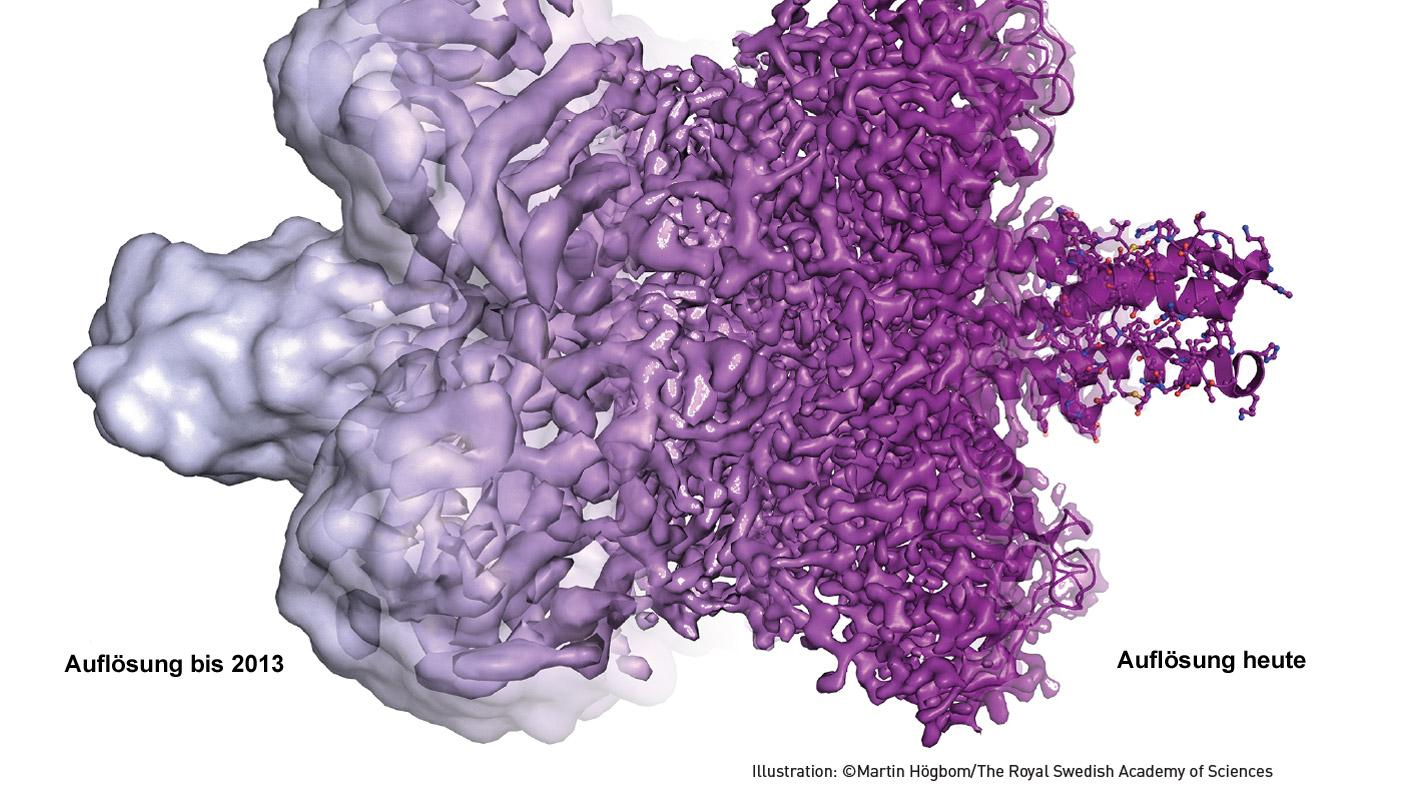
\includegraphics[width=.95\textwidth]{images/Verbesserung_der_Aufloesung.jpg}
    \caption{Verbesserung der Auflösung von 2013 bis heute 2017\protect\footnotemark{}.}
    \label{fig:auflösung}
\end{figure}
\footnotetext{\url{http://www.blopig.com/blog/wp-content/uploads/2014/04/CootLigand2-624x349.png}}



\begin{figure}
    \centering
    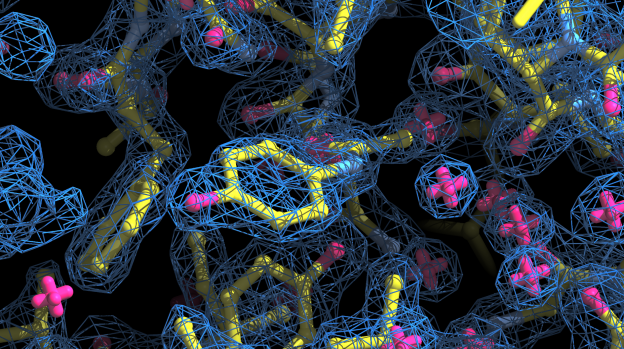
\includegraphics[width=.95\textwidth]{images/approximation.png}
    \caption{Dargestellt ist eine Approximation der Atome eines Proteins.}
    \label{fig:approximation}
\end{figure}




\section{Anwendungsgebiete}

Sollte es möglich sein alle \ac{SNP}s im Illumina... zu annotieren, so ist es denkbar spezielle SNPs im Blut zu suchen.


Rückfall Quote nach Remission

MDS

SNPs im Blut nachweisen

geringe Konzentration



mukl